\documentclass{beamer}
\usepackage{xeCJK}
%\usepackage{newtxtext,newtxmath}	% use Times Roman font
%\usefonttheme{serif}
\usefonttheme{professionalfonts}
%\setbeamertemplate{theorems}[numbered]
\setbeamertemplate{caption}{\insertcaption} 	% no `Figure' prefix before caption

\mode<presentation> {

%\usetheme{default}
%\usetheme{AnnArbor}
%\usetheme{Antibes}
%\usetheme{Bergen}
%\usetheme{Berkeley}
%\usetheme{Berlin}
%\usetheme{Boadilla}
%\usetheme{CambridgeUS}
%\usetheme{Copenhagen}
%\usetheme{Darmstadt}
%\usetheme{Dresden}
%\usetheme{Frankfurt}
%\usetheme{Goettingen}
%\usetheme{Hannover}
%\usetheme{Ilmenau}
%\usetheme{JuanLesPins}
%\usetheme{Luebeck}
\usetheme{Madrid}
%\usetheme{Malmoe}
%\usetheme{Marburg}
%\usetheme{Montpellier}
%\usetheme{PaloAlto}
%\usetheme{Pittsburgh}
%\usetheme{Rochester}
%\usetheme{Singapore}
%\usetheme{Szeged}
%\usetheme{Warsaw}

%\usecolortheme{albatross}
%\usecolortheme{beaver}
%\usecolortheme{beetle}
%\usecolortheme{crane}
%\usecolortheme{dolphin}
%\usecolortheme{dove}
%\usecolortheme{fly}
%\usecolortheme{lily}
%\usecolortheme{orchid}
%\usecolortheme{rose}
%\usecolortheme{seagull}
%\usecolortheme{seahorse}
%\usecolortheme{whale}
%\usecolortheme{wolverine}

%\setbeamertemplate{footline} % To remove the footer line in all slides uncomment this line
%\setbeamertemplate{footline}[page number] % To replace the footer line in all slides with a simple slide count uncomment this line
\setbeamertemplate{navigation symbols}{} % To remove the navigation symbols from the bottom of all slides uncomment this line
}

\usepackage{graphicx} % Allows including images
\usepackage{verbatim} % comments
\usepackage{tikz-cd}  % commutative diagrams
\newcommand{\tikzmark}[1]{\tikz[overlay,remember picture] \node (#1) {};}
\usepackage{booktabs} % Allows the use of \toprule, \midrule and \bottomrule in tables
\usepackage{amssymb}  % \leftrightharpoons

\newcommand{\vect}[1]{\boldsymbol{#1}}
\newcommand*\sigmoid{\vcenter{\hbox{
\includegraphics{sigmoid.png}}}}

\makeatletter
\renewcommand{\boxed}[1]{\fbox{\m@th$\displaystyle\scalebox{0.9}{#1}$} \,}
\makeatother

%---------------------------- make slide margin narrower --------------------------------
%\newcommand\Wider[2][3em]{%
%	\makebox[\linewidth][c]{%
%		\begin{minipage}{\dimexpr\textwidth+#1\relax}
%			\raggedright#2
%		\end{minipage}%
%	}%
%}

%----------------------------------------------------------------------------------------
%	TITLE PAGE
%----------------------------------------------------------------------------------------

\title[Genifer white paper]{Genifer --- white paper} % The short title appears at the bottom of every slide, the full title is only on the title page

\author{YKY 甄景贤} % Your name
\institute[] % Your institution as it will appear on the bottom of every slide, may be shorthand to save space
{
Independent researcher, Hong Kong \\ % Your institution for the title page
\medskip
\textit{generic.intelligence@gmail.com} % Your email address
}
\date{\today} % Date, can be changed to a custom date

\begin{document}

\frame{\titlepage}

%\begin{frame}
%\frametitle{Talk summary}
%\tableofcontents
%\end{frame}

%---------------- this is for when you're using \part's ----------------------------------
%\begin{frame}
%\frametitle{Summary}
%
%{\usebeamerfont*{frametitle} Part I %\usebeamercolor[fg]{frametitle}
% ~ ~ ~ Deep reinforcement learning}
%%\tableofcontents[part=1]
%
%\vspace{1.5cm}
%{\usebeamerfont*{frametitle} Part II %\usebeamercolor[fg]{frametitle}
% ~ ~ ~ Logical structure}
%%\tableofcontents[part=2]
%\end{frame}

%----------------------------------------------------------------------------------------
%	PRESENTATION SLIDES
%----------------------------------------------------------------------------------------

%------------------------------------------------

\part{title}\begin{frame}
\frametitle{The missing link in strong AI}
\begin{itemize}
\item Classical (predicate) logic captures human intelligence, but its learning algorithm (inductive logic programming, based on discrete, combinatorial search) is \textit{too slow}.
\item Deep learning is fast but we don't know how to design \textit{neural representations}.
\end{itemize}
\begin{equation}
\vcenter{\hbox{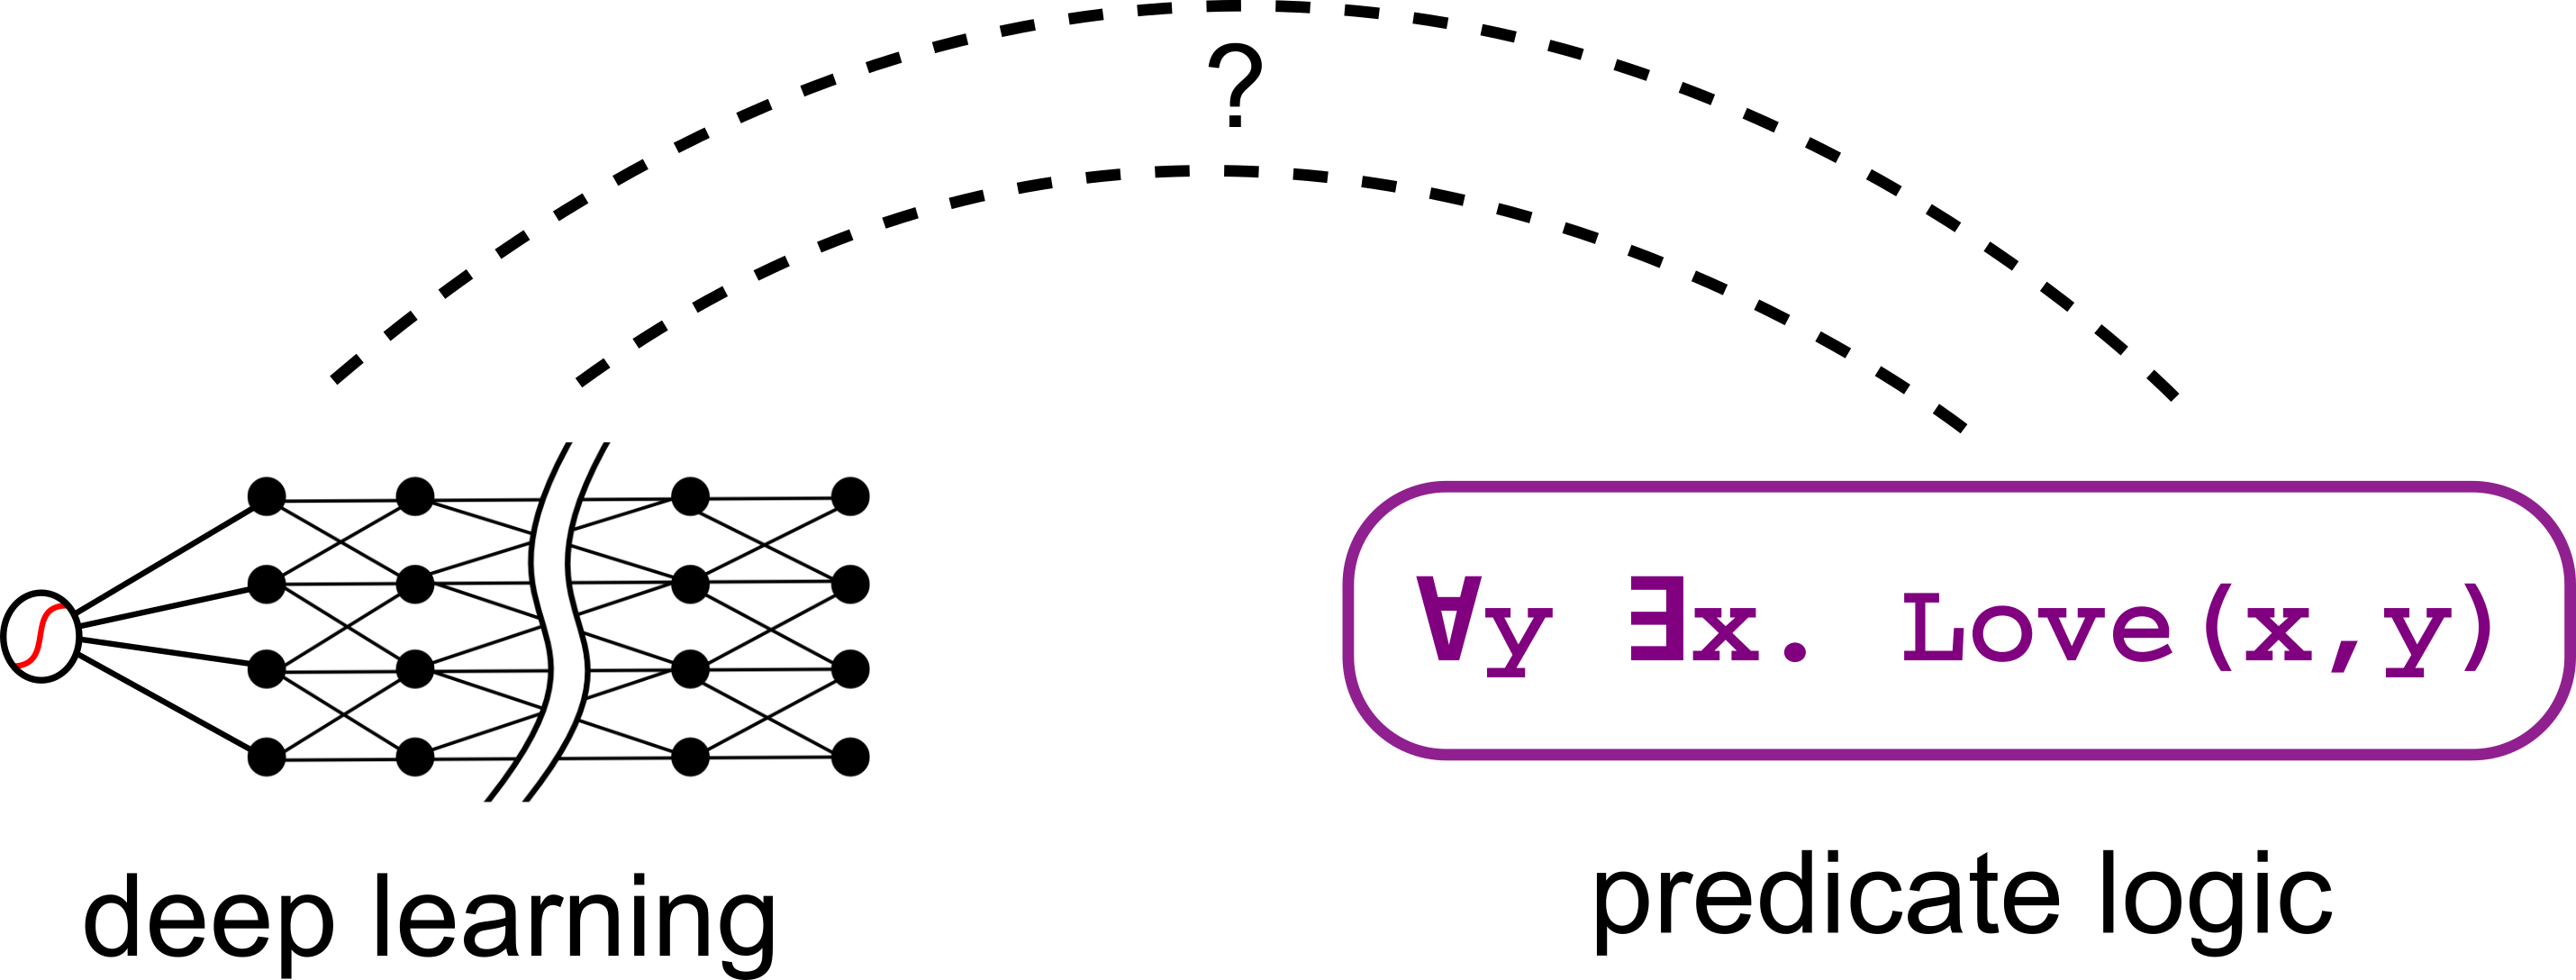
\includegraphics[scale=0.65]{AGI-missing-link-0.png}}}
\end{equation}
\end{frame}

\begin{frame}
\frametitle{The problem with predicate logic}
\begin{equation}
\forall x,y,z. \; \mbox{father}(x,y) \wedge \mbox{father}(y,z) \rightarrow \mbox{grandfather}(x,z)
\end{equation}
\begin{itemize}
	\item This involves \textbf{variable substitutions} which are troublesome to handle with neural networks. \\
	(The difficulty seems to come from the cylindric-algebraic structure of predicate logic:  if a formula have variables $x_1, x_2, x_3, ...$, we would need to consider the domain $D \times D \times D \times ...$ where $D \ni x_i$)
\end{itemize}
\end{frame}

\begin{frame}
\frametitle{Relation algebra}
Given that:
\begin{equation}
\mbox{Father} \circ \mbox{Father} = \mbox{Grandfather}
\end{equation}
we can deduce:
\begin{eqnarray}
\mbox{john Father paul} \\
\mbox{paul Father pete} \\
\Rightarrow \mbox{john Father $\circ$ Father pete} \\
\Rightarrow \mbox{john Grandfather pete}
\end{eqnarray}
via \textit{direct} substitution of equal terms.
\begin{itemize}
	\item  Relation algebra appears very \textit{natural} and similar to human thinking
\end{itemize}
\end{frame}

\begin{frame}
\frametitle{The solution: term rewriting systems}
\begin{itemize}
	\item The essence of relation algebra seems to be \textbf{sequence-rewriting} (though relation algebra has other operations)
	\item I believe sequence-rewriting is the missing link between ``neural'' and logic. 
\end{itemize}
\begin{equation}
\vcenter{\hbox{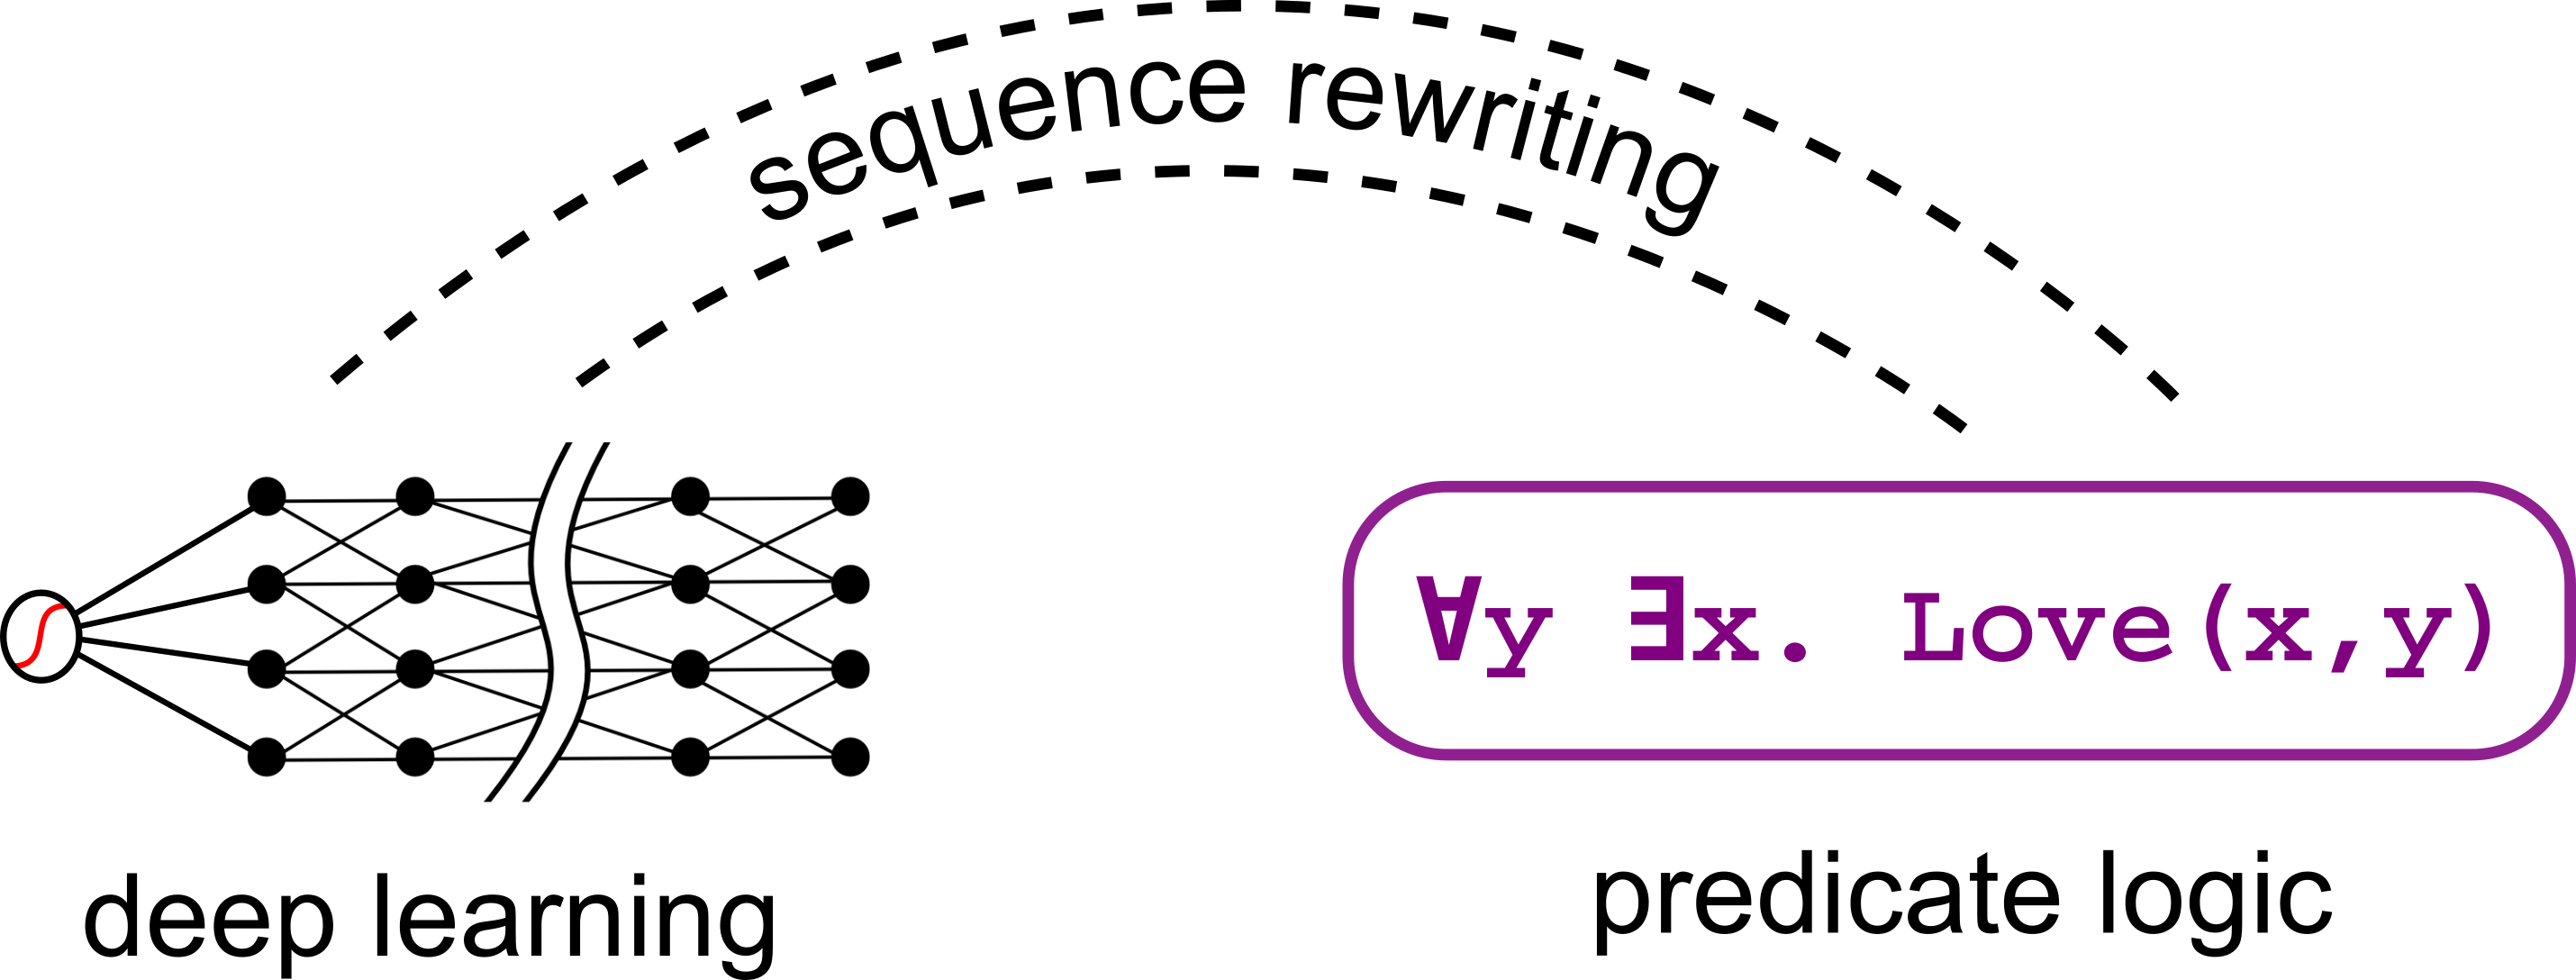
\includegraphics[scale=0.65]{AGI-missing-link.png}}}
\end{equation}
\end{frame}

\begin{frame}
\frametitle{Sequence to sequence}
Sequence to sequence:
\begin{equation}
\boxed{A}\boxed{B}\boxed{C}\boxed{D} \rightarrow \boxed{X}\boxed{Y}\boxed{Z}
\end{equation}
\textbf{Sequence-of-sequences} to sequence:
\begin{equation}
\label{eqn:SoS2S}
\boxed{A}\boxed{B}\boxed{C}\boxed{D} \wedge \boxed{E}\boxed{F}\boxed{G} \rightarrow \boxed{X}\boxed{Y}\boxed{Z}
\end{equation}
Note the similarity between (\ref{eqn:SoS2S}) and \textit{logical reasoning}.
\begin{itemize}
	\item We already know that RNN is good at sequence-to-sequence processing
	\item How to design RNN to do sequence-of-sequences-to-sequence?
\end{itemize}
\end{frame}

\begin{frame}
\frametitle{RNN for seq-of-seqs-2-seq}
I'm not 100\% sure if it would work, but this is one idea:

Sequence to sequence:
\begin{equation}
\vcenter{\hbox{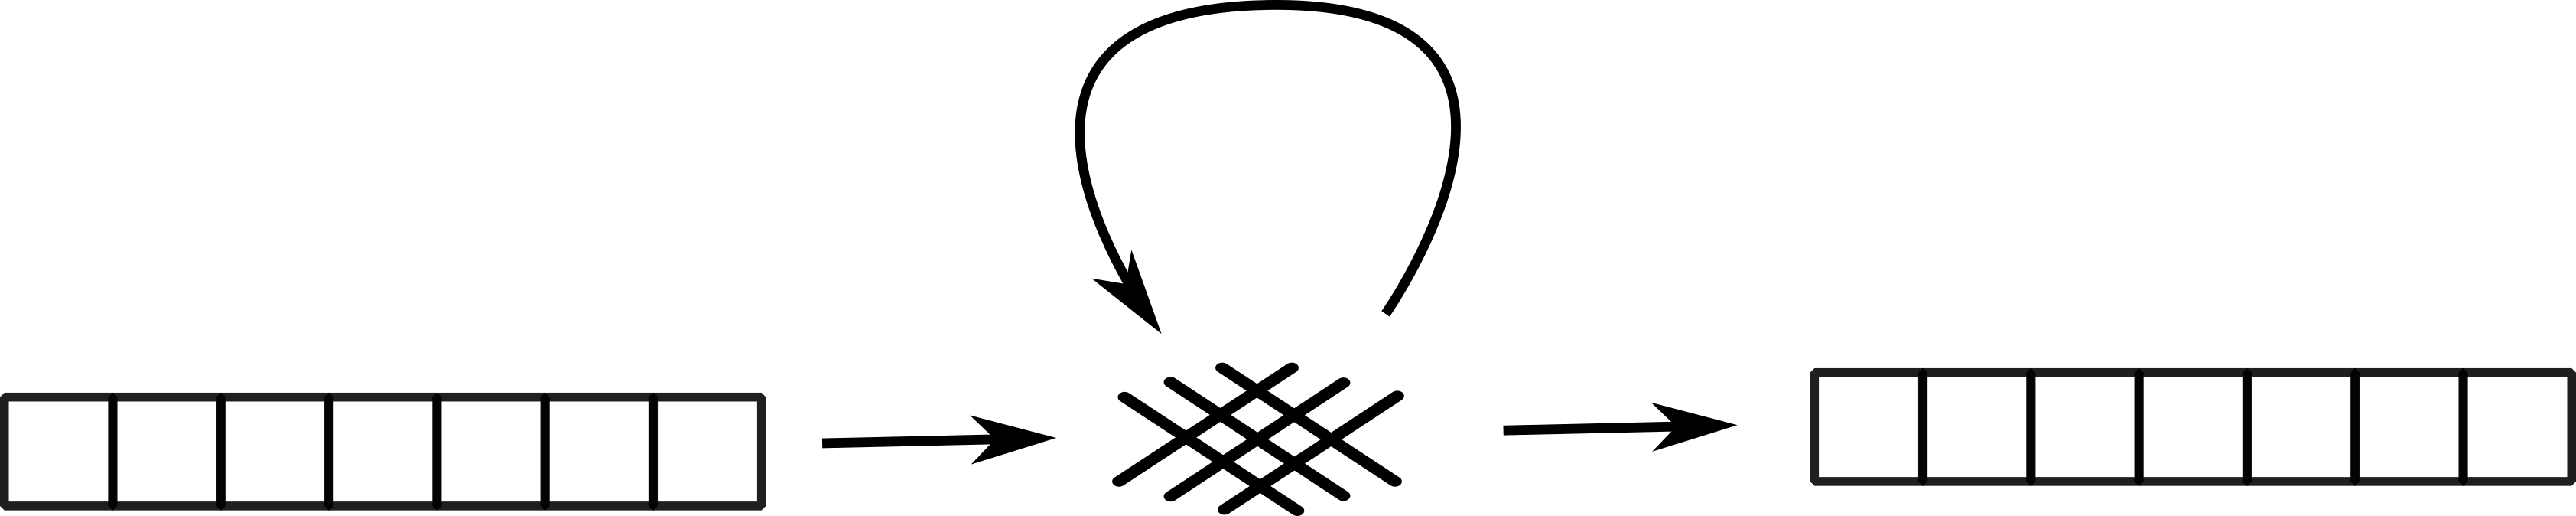
\includegraphics[scale=0.5]{RNN-seq-2-seq.png}}}
\end{equation}
Sequence-of-sequences to sequence:
\begin{equation}
\label{eqn:RNN-architecture}
\vcenter{\hbox{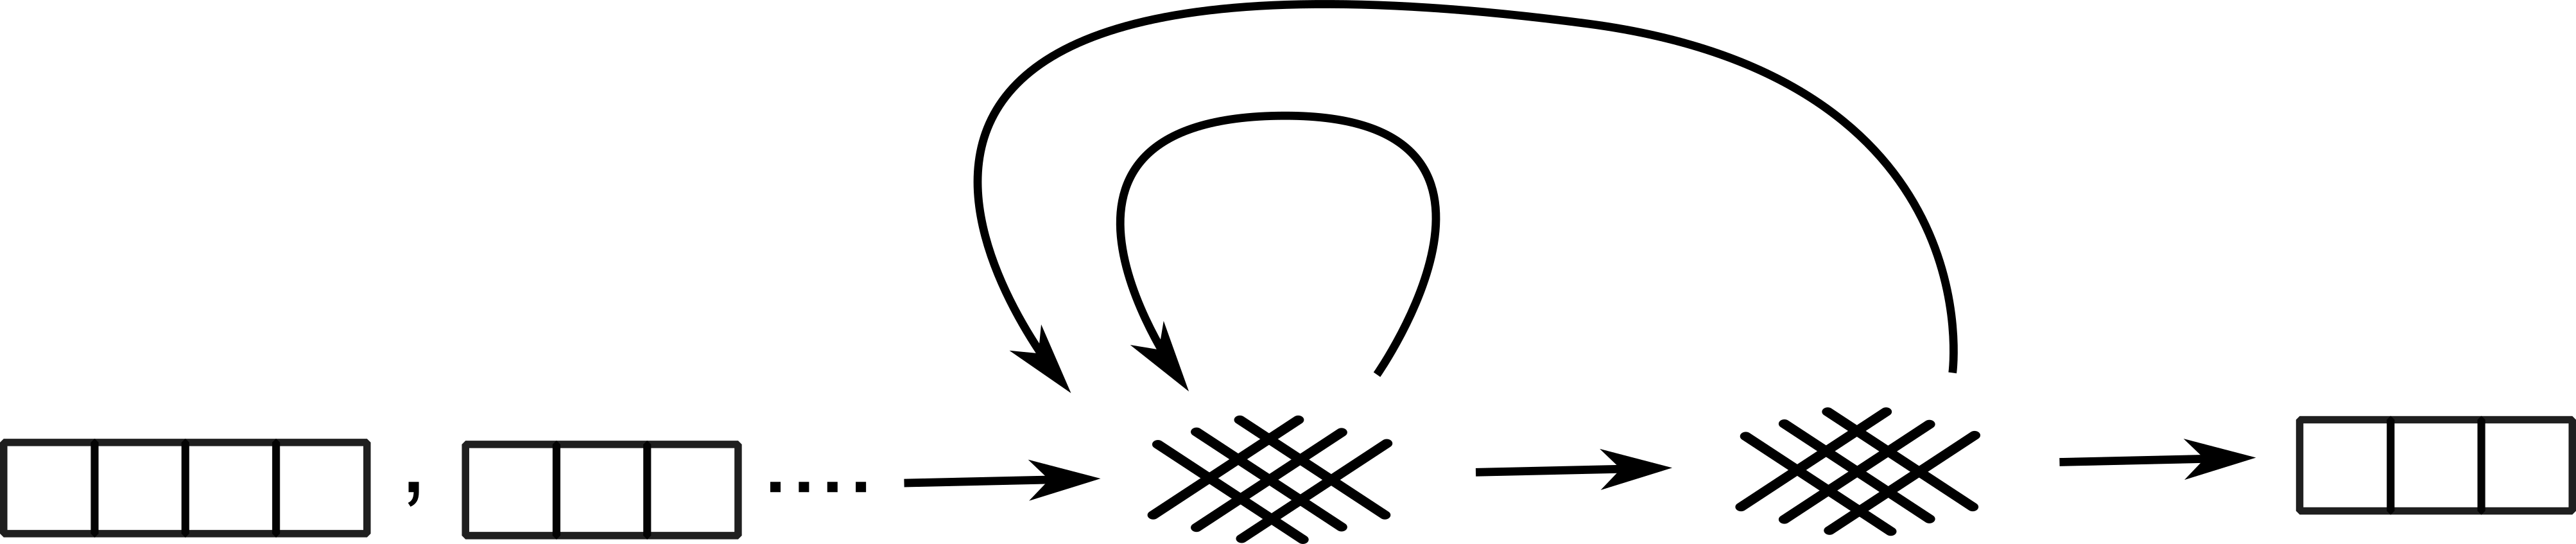
\includegraphics[scale=0.5]{RNN-seq-of-seqs-2-seq.png}}}
\end{equation}
\end{frame}


%\cite{Jacobs1999}

\begin{comment}

\begin{frame}
\frametitle{References}
\footnotesize{
\begin{thebibliography}{99} % Beamer does not support BibTeX so references must be inserted manually as below
\bibitem[]{} Bart Jacobs (1999)
\newblock Categorical logic and type theory
% \newblock \emph{North Holland, Studies in logic} v141.

\bibitem[]{} Robert Goldblatt (2006)
\newblock Topoi -- the categorical analysis of logic

\end{thebibliography}
}
\end{frame}
\end{comment}

\begin{frame}
It may look simple, but I think the RNN architecture (\ref{eqn:RNN-architecture}) is sufficient for AGI.  We're looking for Tensorflow developers to implement a prototype.

\vspace*{1cm}
\Large{\centerline{Thank you}}

%\vspace*{1cm}
%\Large{\centerline{The End}}
\end{frame}

\end{document} 